\section{Context and system overview}

We start this section by presenting an abstract machine, \textit{banzai} that
captures several important features of programmable switch
architectures~(\S\ref{ss:abstract}) with deterministic performance. We use
banzai as the compiler target throughout the paper and later
discuss~(\S\ref{s:p4}) how targeting P4 would allow domino to run on
programmable switching chips.

\subsection{Banzai: An abstract machine for programmable switches}
\begin{figure*}[!t]
  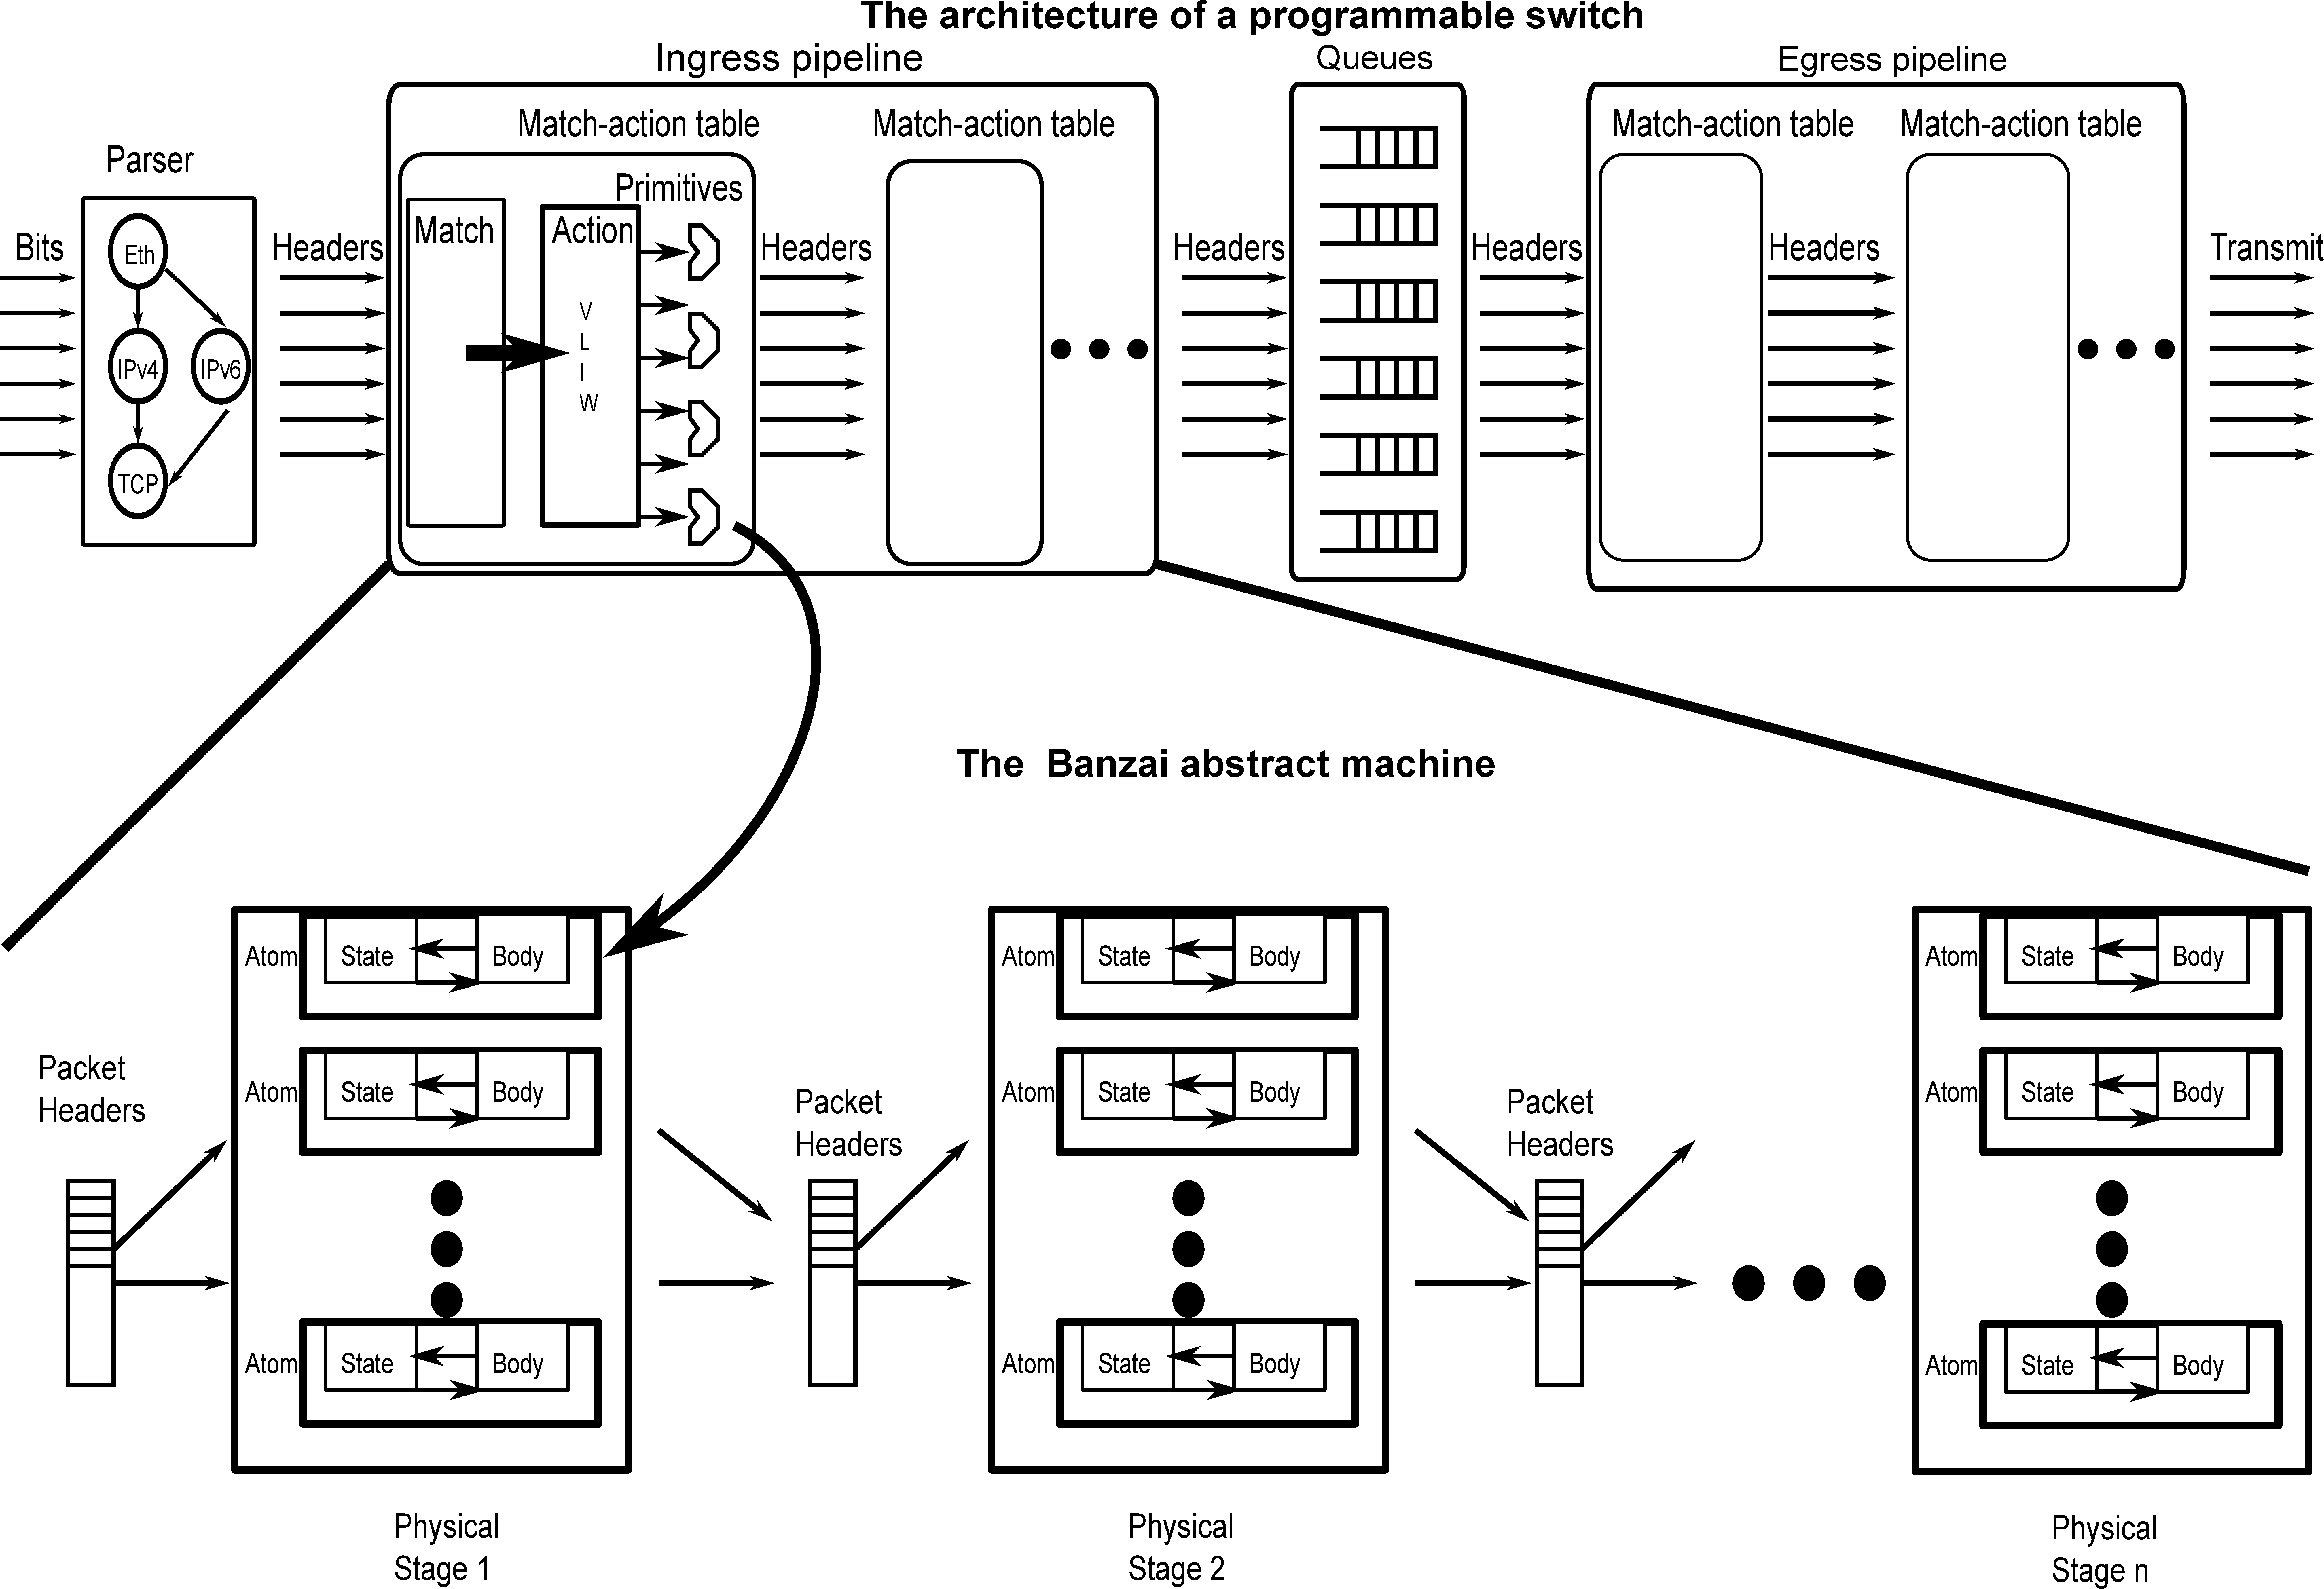
\includegraphics[width=\textwidth]{banzai.pdf}
  \caption{The Banzai abstract machine and its relationship to programmable switch architectures.}
  \label{fig:switch}
\end{figure*}
Our abstract machine is directly inspired by programmable switch architectures
such as the Reconfigurable Match-Action Table architecture (RMT), Intel's
FlexPipe, and Cavium's XPliant. These architectures assume a switch model
(Figure~\ref{fig:switch}) that consists of an ingress pipeline, followed by the
switch scheduler, followed by an egress pipeline.

banzai is an abstract machine that models either of these two pipelines, with
the only difference being the packet fields available at the entrance of these
pipelines. Being an abstract machine, banzai only models mechanisms that are
critical to mapping data-plane algorithms. In particular, it models the
computation that happens in each match-action table (i.e. the action half of
the match-action table). Notably, banzai doesn't model packet parsing nor the
matching semantics of each match-action table (direct, ternary, or LPM).

A switch pipeline in banzai has a number of pipeline stages that execute in
parallel. Each stage contains a vector of \textit{atoms}, with the atoms
themselves executing in parallel. Informally, an atom is an atomic unit of
packet processing and is represented by a body of imperative code that executes
sequentially. An atom is assumed to complete execution and modify a packet
before the next packet is processed by that atom.

An atom may also contain internal state that can influence the atom's behavior
from one packet to the next and persists across packets. For instance, a switch
counter could be written as an atom as follows\footnote{We use the notation p.x
  to represent access to field ``x'' within a packet p and the notation x to
represent access to the state variable ``x'' that persists across packets}.
\begin{verbatim}
  p.tmp     = counter;
  p.tmp2    = p.tmp + 1;
  counter   = p.tmp2;
\end{verbatim}
Similarly, a stateless operation that sets a packet field, such as the
modify\_field action primitive in P4 (equivalently, the bitmasked-set operation
from the RMT architecture) can be written as the atom below:
\begin{verbatim}
  p.field   = value;
\end{verbatim}

The banzai abstract machine generalizes several aspects of a programmable
switch architecture. The vector of atoms in each stage generalizes RMT's
very-large instruction-word (VLIW)~\cite{rmt} that executes primitive actions
on independent packet fields in parallel. The presence of internal state in an
atom models persistent switch state residing on a switch such as meters,
counters, , and P4's register abstraction in a unified manner.

\textbf{Performance constraints on atoms} \\

Any switch hardware that is expected to run at line rate will need to constrain
atoms to bound the execution latency of each atom and provide deterministic
performance regardless of the computations carried out by each atom. We impose
two such constraints that distinguish banzai from software packet-processing
platforms such as Click and Network Processors such as the Intel IXP, which
tradeoff deterministic performance for greater flexibility in expressing packet
processing code.

First, banzai is a shared-nothing architecture: state variables are internal to
a particular atom and their values can only be communicated with atoms in
subsequent stages by writing these state variables into packet fields that are
then read downstream.  This restriction reflects the capabilities of most
switches today: building memories that can be simultaneously accessed from
multiple switch stages is technically challenging.

%%To let a stage communicate state information to a predecessor stage upstream,
%%banzai allows packets to be cloned and recirculated back into a pipeline,
%%modeling the loopback interfaces found on most switches today.
Second, we constrain the complexity of atom bodies by definining how atoms are
executed. One execution model is an in-order CPU that can execute at most $N$
instructions sequentially. Another is a configurable combinational circuit in
hardware~\cite{dataflow}, where the circuit limits the space of feasible
computations and needs its control signals to be configured to match the
behavior of the atom.

We use both models in this paper. For stateless atoms that don't modify state,
we constrain atom bodies to consist of only statements that can be represented
as three-instruction codes. Further, we allow exactly one statement in each
atom body. This roughly corresponds to the set of primitive actions available
in P4/RMT.  For atoms that do modify state, we consider both models
(\S\ref{s:constraints}) and evaluate how atom body constraints affect whether
or not packet-processing code can be mapped onto banzai.

% --> Packet transactions and how this is different from other transactions.
\subsection{Packet transactions}
\begin{figure}
  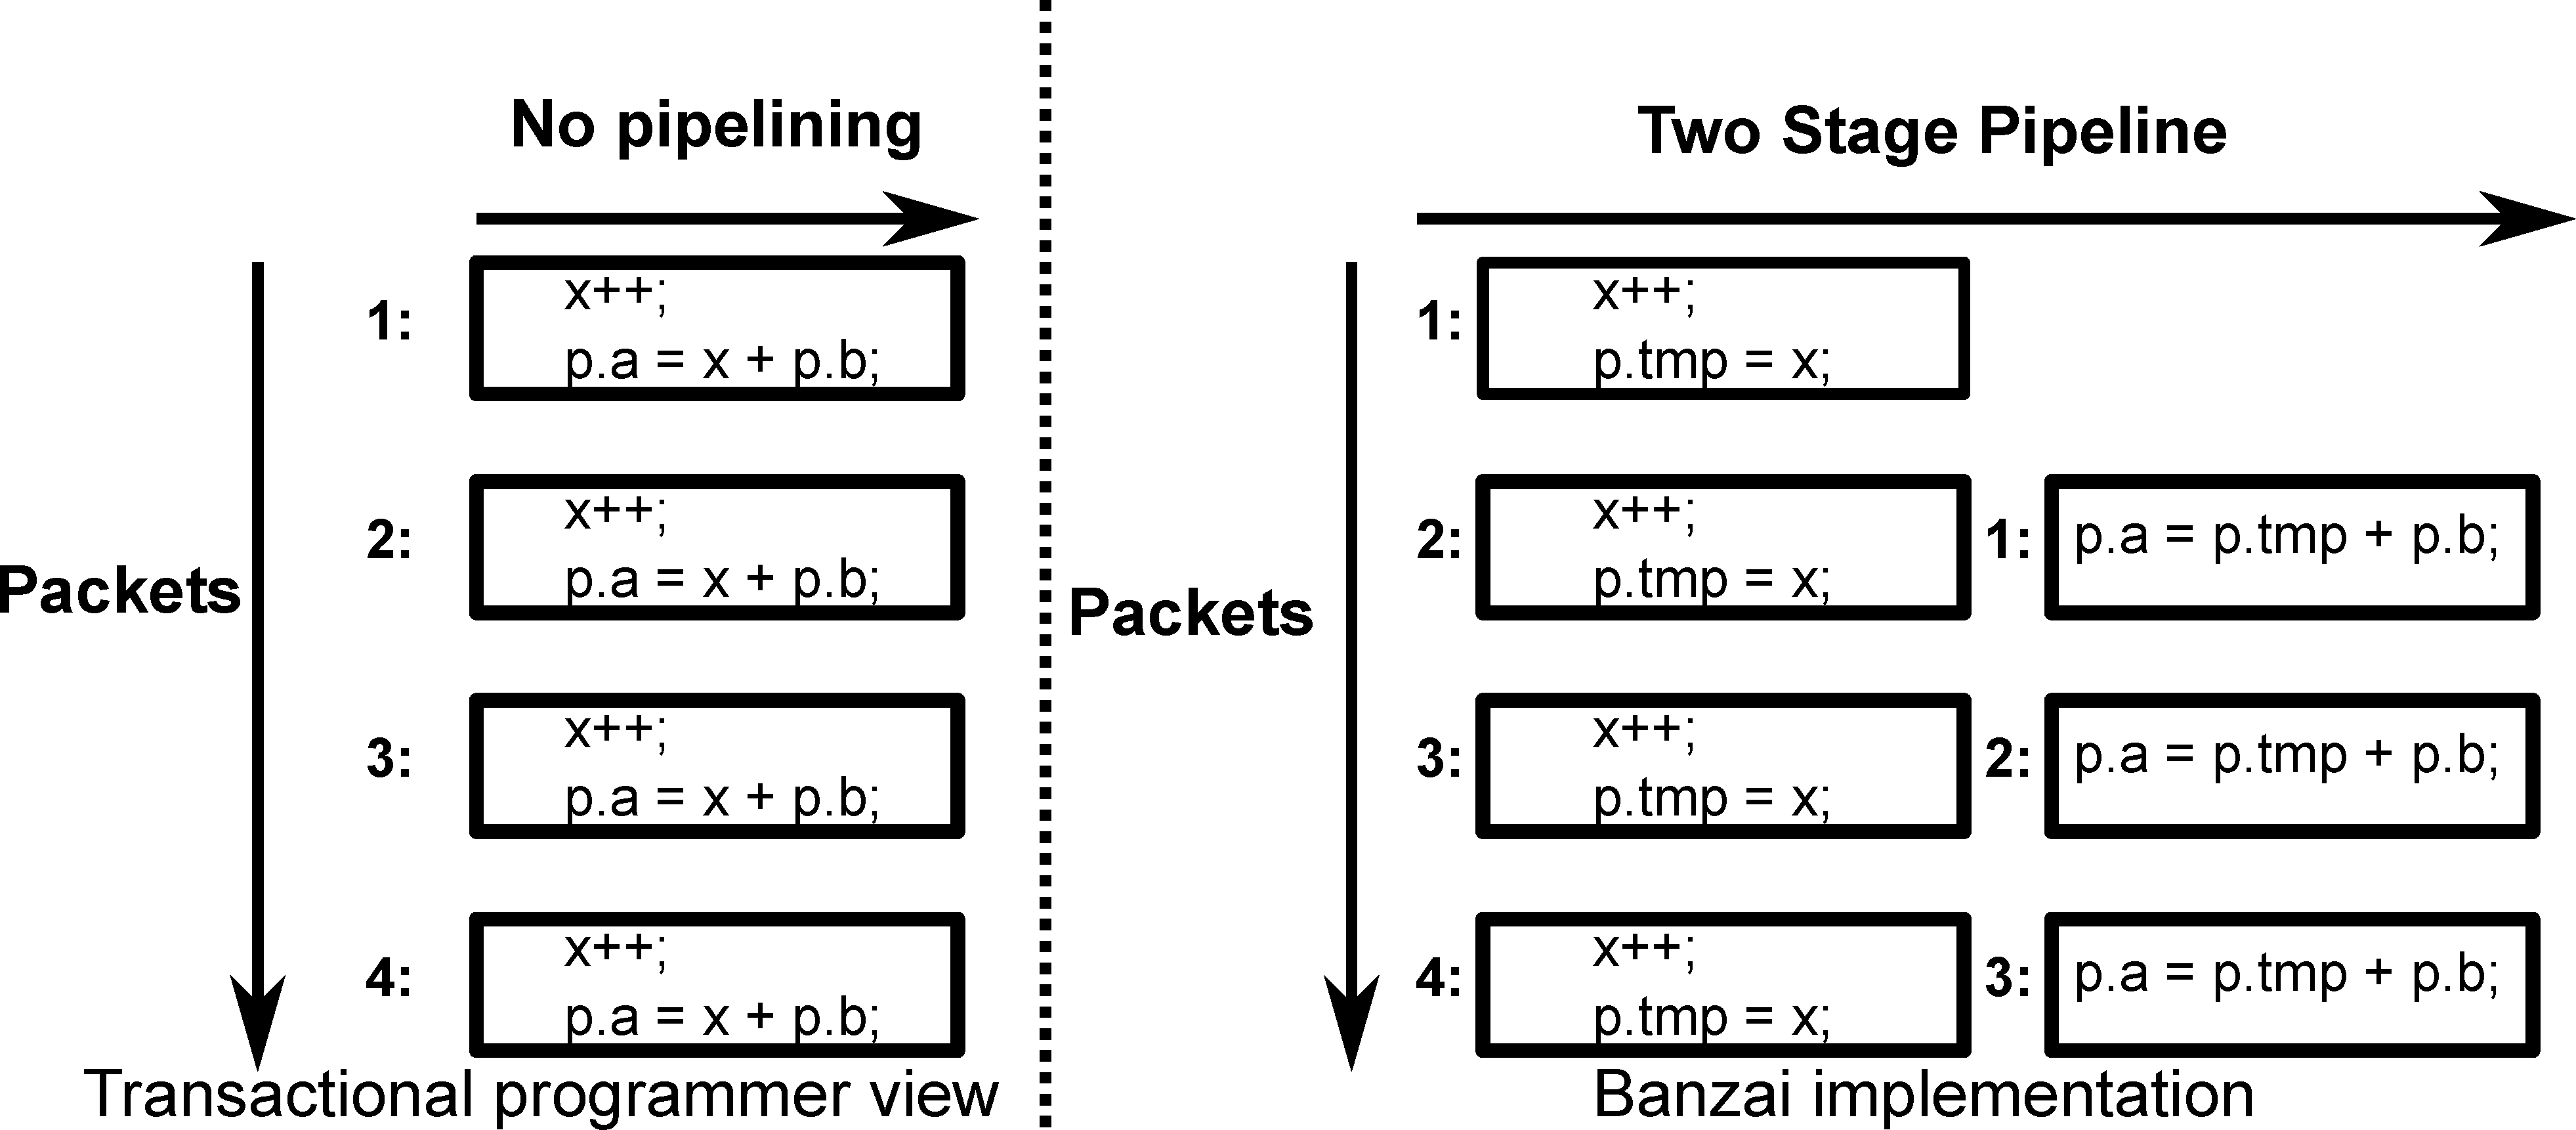
\includegraphics[width=\columnwidth]{spec_vs_impl.pdf}
  \caption{A packet transaction and its implementation}
  \label{fig:trans}
\end{figure}

Having described our target architecture, we now describe a programming model
for it, inspired by database transactions. Transactions are the strongest
guarantee that a database system can provide in that the effect of a
transaction is either entirely visible or not with no intermediate state being
visible to the outside world.

We repurpose database transactions for data-plane programming by defining the
notion of a \textit{packet transaction}: a body of sequential code that
executes from start to finish on each packet and conceptually processes only
one packet at a time. For a programmer, the packet transaction represents
exactly what happens to every packet. Every packet is processed in isolation
and to completion before the next packet's processing begins.
% TODO: Show how each packet is processed to completion in the transactional world,
% while packets are interleaved in the pipelined world.

In practice though, switch hardware is heavily pipelined
(Figure~\ref{fig:switch}).  A compiler automatically translates the
programmer's transactional code block into a low-level pipelined implementation
on the switch hardware (Figure~\ref{fig:trans}).

Put differently, the user's packet transaction is a single atom that captures
all computations on the packet and encapsulates all the state required to carry
out the computation.  A compiler then translates this packet transaction into
into a grid of atoms that is functionally equivalent to the single atom, while
respecting hardware constraints on each atom's complexity. If the compiler is
unable to find a mapping, it rejects the packet transaction as being too
complex for the given target.
